\section{Etape 1}
\subsection{Objectifs}

L'objectif de ce projet fil rouge est de permettre la mise en place d'une infrastructure de communication.
Il nous permettra de décrouvrir, étudier et mettre en place différents protocoles de communication. Cette première étape 
consiste à faire passer une information entre une source et une destination en utilisant
un transmetteur parfait. Grâce à cela nous découvrirons l'architecture logicielle proposée pour ce projet. Nous en profiterons également
pour commencer la mise en place de test utilisant JUnit afin d'assurer le fonctionnement des différents composants du système.

\subsection{Choix d'implémentation}

\pagebreak

\subsection{Sondes}

Lors de l'execution de la commande: 

\begin{figure}[h]
    \centering
    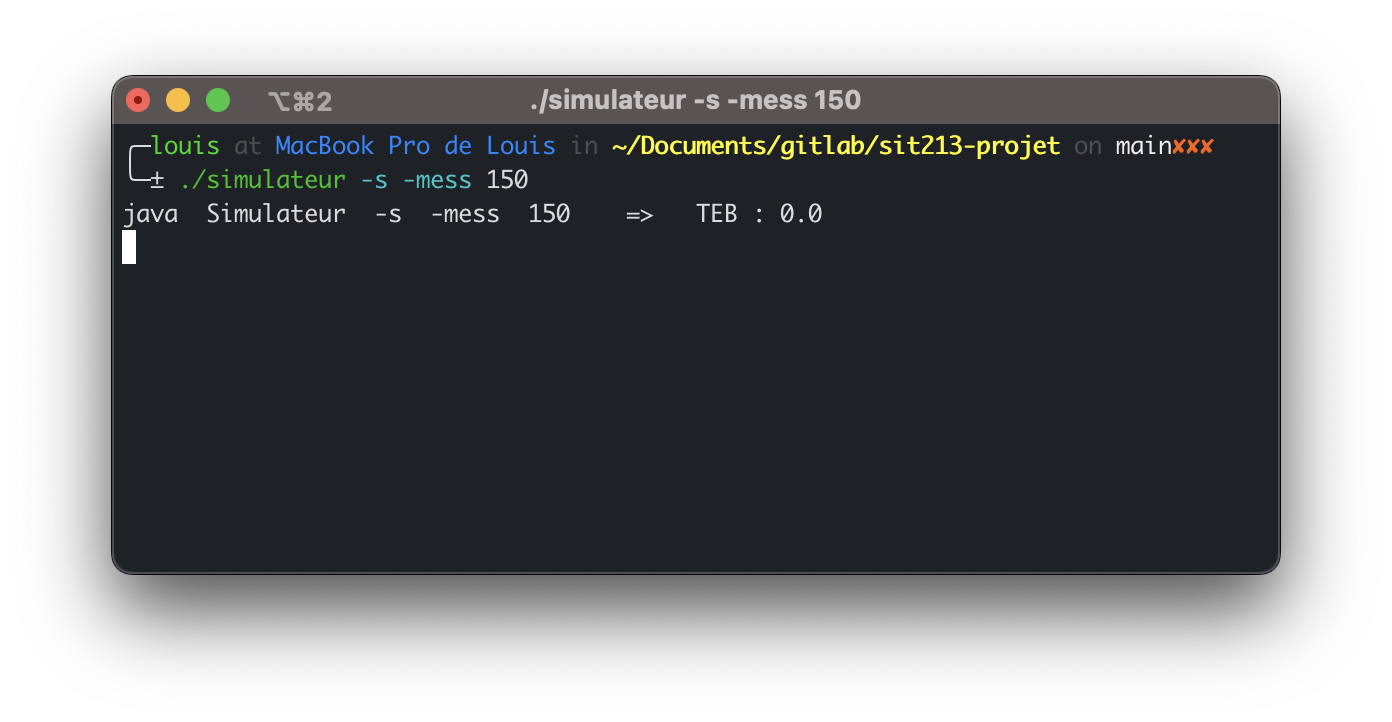
\includegraphics[width=\textwidth]{term_1.png}
    \caption{terminal}
\end{figure}

On constate lors de l'execution du script l'affichacge d'un signal identique sur la source et la destination (voir figure 2). Cela coincide 
avec le fait que le transmetteur est parfait et que le signal n'est donc pas modifié lors de la transmission vers la destination.

\begin{figure}[h]
    \centering
    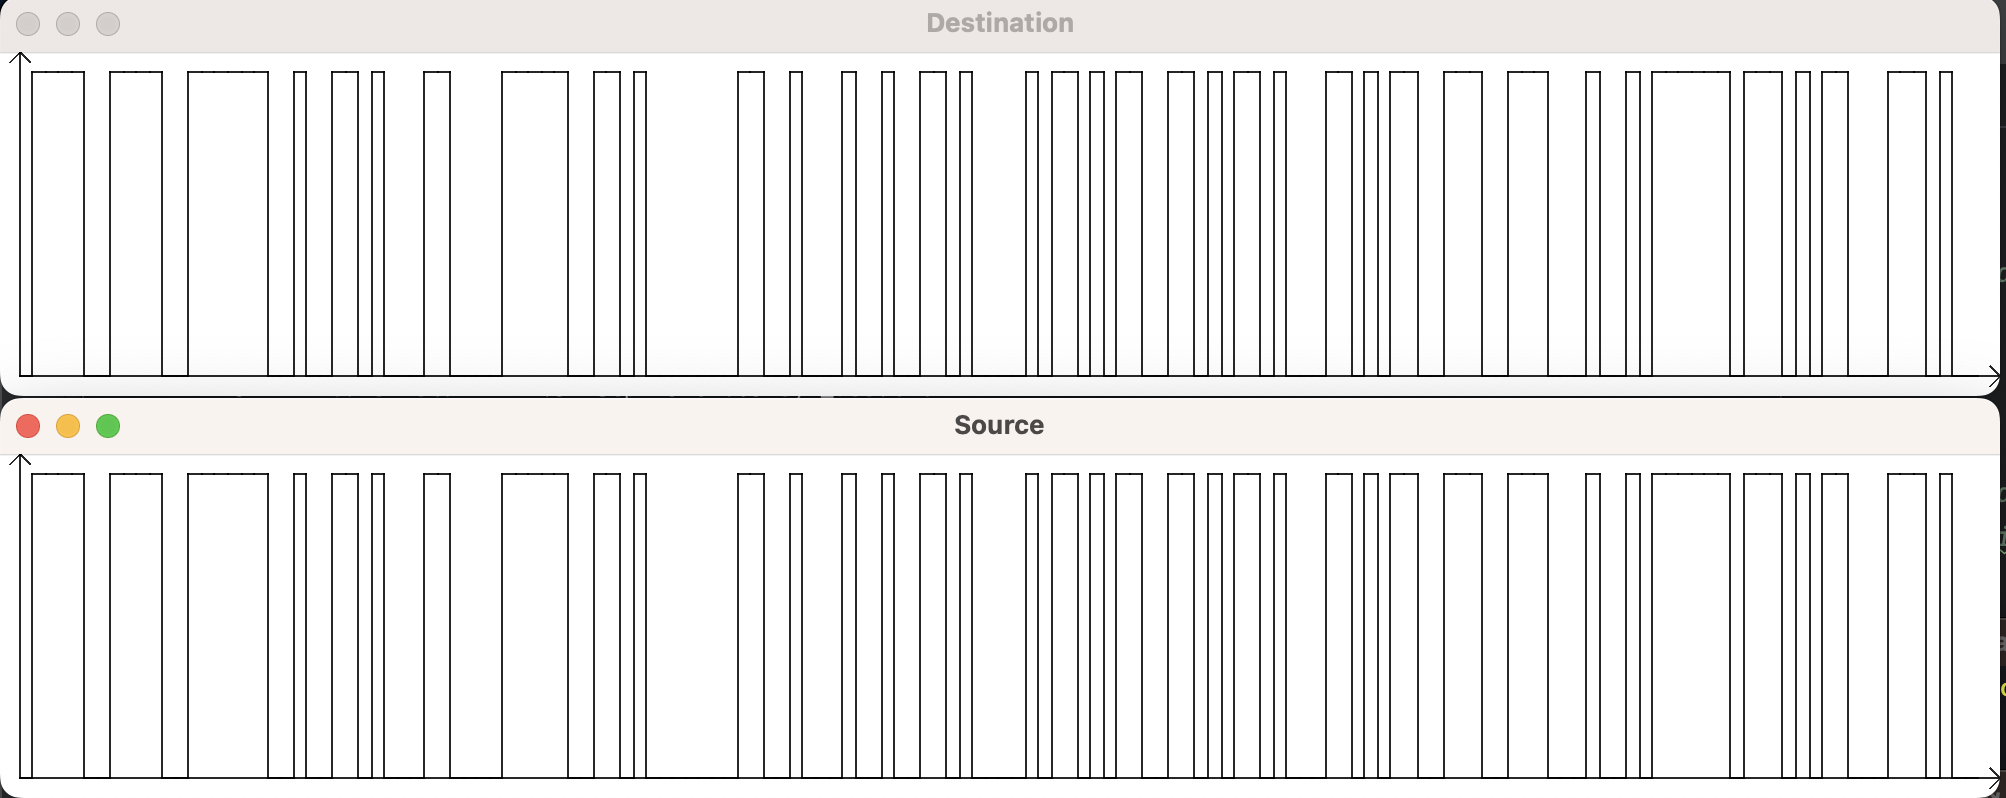
\includegraphics[width=\textwidth]{s_r_100.png}
    \caption{Sondes}
\end{figure}
\subsection{Performances}

\subsubsection{Conclusion}
% \begin{lstlisting}
    
    
% \end{lstlisting}

